\newpage
\section{Order}
Orders are a new feature in Salespoint 2011. The intention was to prepare the old databaskets for development of web applications and extend them to collaborate with our new inventory, providing the opportunity of individual pricing, final payment and basic log functionality.

Therefore we created the \code{OrderEntry} as main data structure to access these functionality. An OrderEntry represents one order and can be imagined as sheet of paper which basically consists of lines representing the ordered products (\code{OrderLine}) and lines that are not bound to a concrete product but which cause charge (\code{ChargeLine}). ChargeLines make it possible to add individual charge to orders. For example they can be used to define forwarding charges or other special charges produced by this order. 

\vskip 1cm

\begin{figure}[ht]
	\centering
  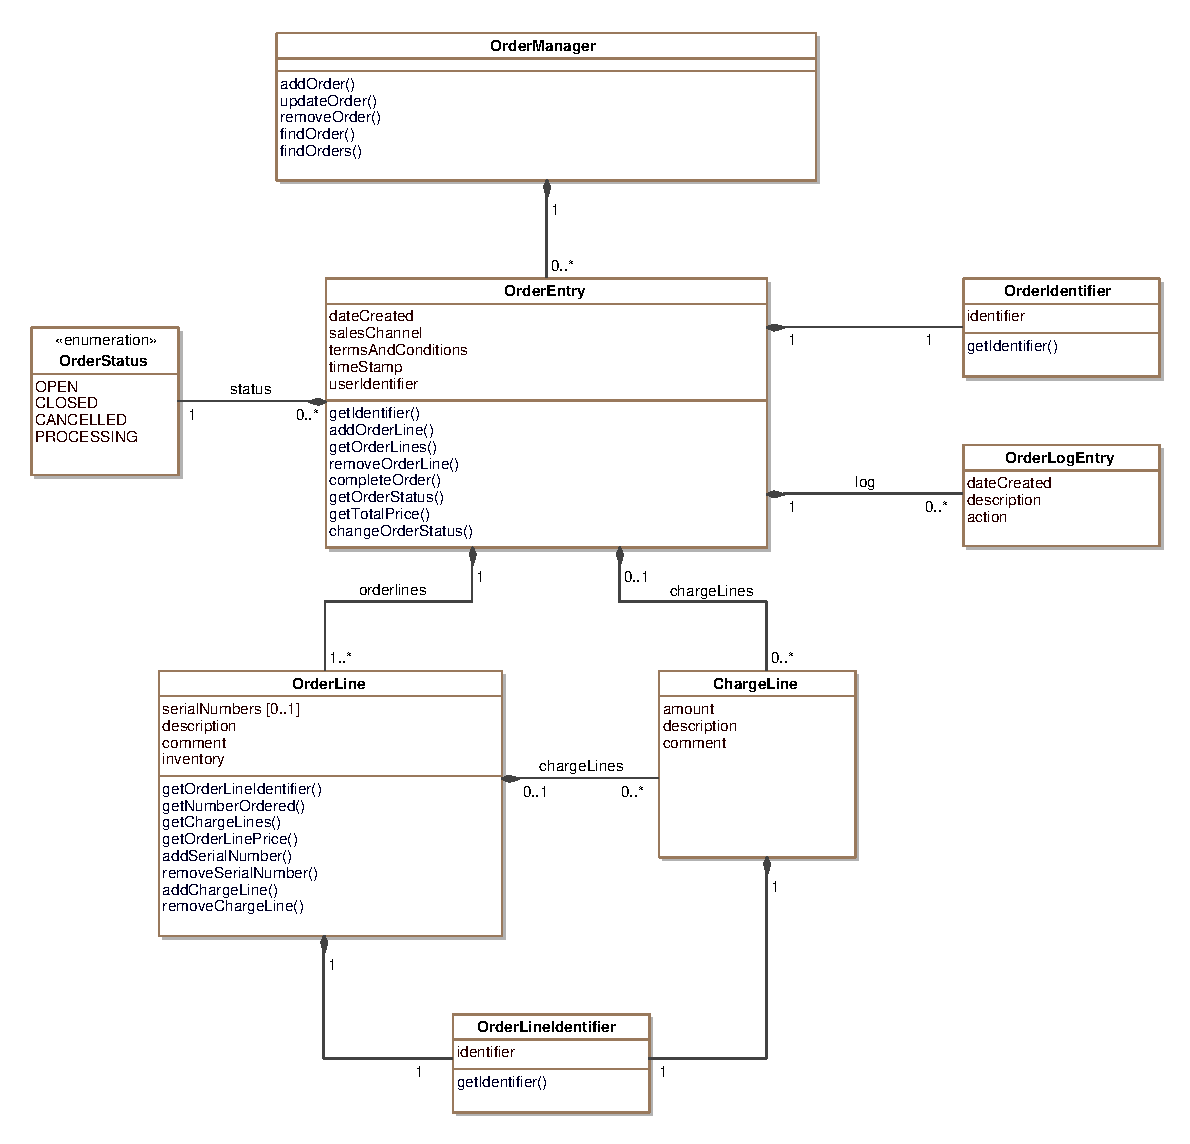
\includegraphics[scale =.7]{images/Overview_Order.eps}
	\label{order_overview}
	\caption{Order - Class Overview}
\end{figure}


